\documentclass[aspectratio=169]{beamer}
\usetheme{Madrid}
\usecolortheme{default}

%% USEPACKAGES %%
\usepackage{subcaption}
\usepackage{csquotes}
\usepackage{datetime}
\usepackage[british]{babel}
\usepackage{tikz}
\usetikzlibrary{positioning, arrows.meta, fit, calc}
\usepackage{tikz-cd}

\usepackage[backend=biber]{biblatex}
\addbibresource{references.bib}

\usepackage{nameref}
\makeatletter
\newcommand*{\currentname}{\@currentlabelname}
\makeatother

\usepackage{subcaption}
\usepackage{pgffor}
\usepackage{listings}
\usepackage{lipsum}
\definecolor{codegreen}{rgb}{0,0.6,0}
\definecolor{codegray}{rgb}{0.5,0.5,0.5}
\definecolor{codepurple}{rgb}{0.58,0,0.82}
\definecolor{backcolour}{rgb}{0.95,0.95,0.92}

\lstdefinestyle{mypython}{
    backgroundcolor=\color{backcolour},
    commentstyle=\color{codegreen},
    keywordstyle=\color{magenta},
    numberstyle=\tiny\color{codegray},
    stringstyle=\color{codepurple},
    basicstyle=\ttfamily\footnotesize,
    breakatwhitespace=false,
    breaklines=true,
    captionpos=b,
    keepspaces=true,
    numbers=left,
    numbersep=5pt,
    showspaces=false,
    showstringspaces=false,
    showtabs=false,
    tabsize=2,
}
\lstset{language=Python,
  style=mypython}

%% BEAMER CONFIG %%
\definecolor{uosblue}{RGB}{1,91,130}
\definecolor{gradient1}{RGB}{2, 110, 156}
\definecolor{gradient2}{RGB}{0, 72, 104}
\setbeamercolor{author in head/foot}{fg=white, bg=gradient1}
\setbeamercolor{title in head/foot}{fg=white, bg=uosblue}
\setbeamercolor{date in head/foot}{fg=white, bg=gradient2}
\setbeamercolor{section in head/foot}{fg=white, bg=uosblue}
\setbeamercolor{titlelike}{fg=white,bg=uosblue}

\setbeamertemplate{item}{bg=uosblue}
\setbeamertemplate{enumerate items}[default]
\setbeamertemplate{itemize items}[default]
\setbeamerfont{title}{series=\bfseries}
\setbeamercolor*{palette primary}{fg=white,bg=uosblue}
\setbeamercolor*{palette secondary}{fg=white, bg=uosblue}
\beamertemplatenavigationsymbolsempty


\AtBeginSection[]
{
    \begin{frame}
        \frametitle{}
        \centering
        \huge{\currentname}
    \end{frame}
}

%% DOCUMENT INFO %%
\title[Compiling SNNs]
{NIR2FPGA: Compiling Spiking Neural Networks into RTL}


\author[Michail Rontionov] % (optional, for multiple authors)
{Michail Rontionov}

\institute[] % (optional)
{
  University of Southampton
}



\newdateformat{monthyeardate}{%
  \monthname[\THEMONTH] \THEYEAR}

\date{\monthyeardate\today}

\titlegraphic{
\includegraphics[height=1.5cm]{img/uos.png}}


\begin{document}
\frame{\titlepage}

\begin{frame}
\frametitle{Table of Contents}
\tableofcontents
\end{frame}



\begin{frame}{Hypothesis 1}
  \begin{columns}
    \centering
    \begin{column}{.4\textwidth}
      \begin{block}{$H_1$}
        In the context of neuromorphic FPGA/ASIC co-design, it is \textbf{enough to implement the primitives and connections} between them to \textbf{describe the majority of} high-level \textbf{SNNs} whilst meeting a given accuracy metric.
      \end{block}
    \end{column}
    \begin{column}{.5\textwidth}
      \centering
      \only<2>{
        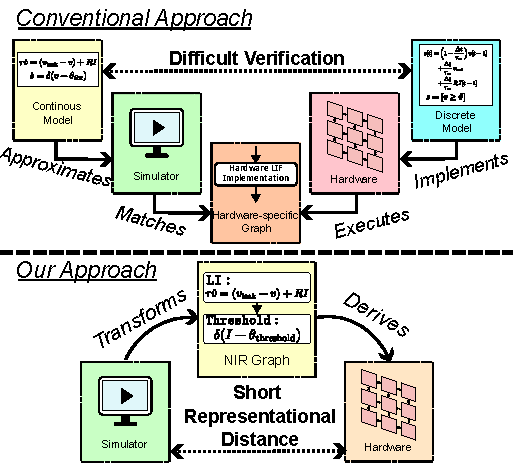
\includegraphics[width=\textwidth]{img/flow.pdf}
      }
    \end{column}
  \end{columns}
\end{frame}

% \begin{frame}{Hypotheses}
%   \begin{block}{$H_1$}
%     In the context of neuromorphic FPGA/ASIC co-design, it is enough to implement the primitives and connections between them to describe the majority of high-level SNNs whilst meeting a given accuracy metric.
%   \end{block}
%   \begin{block}{$H_2$}
%     NIR is an effective \emph{type system} for spiking neural networks executing in various computational spaces, allowing for effective and robust optimisations across each transformation.
%   \end{block}
% \end{frame}

\begin{frame}{(Future) Publication}
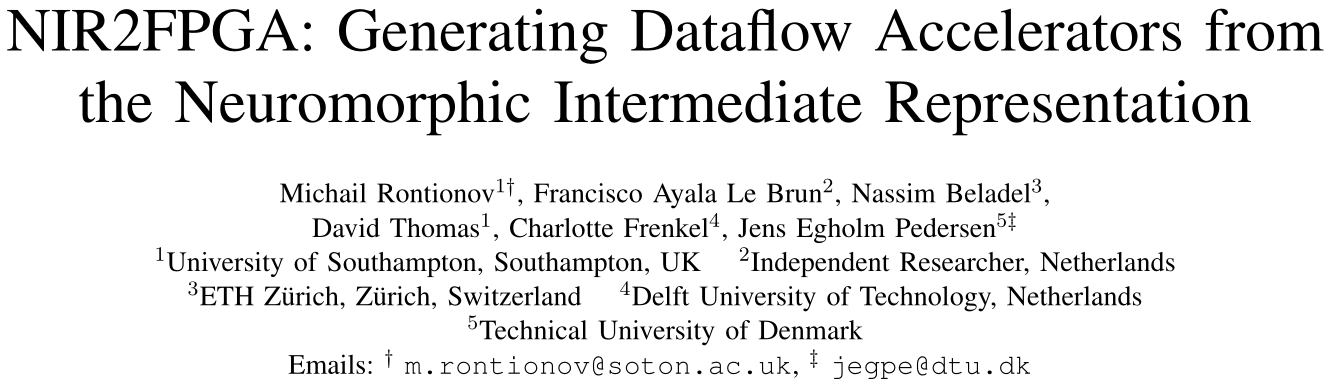
\includegraphics[width=\textwidth]{img/nir2fpga.png}
\end{frame}

\begin{frame}{What does it do?}
  \begin{columns}
    \begin{column}{.8\textwidth}
      \begin{itemize}[<+->]
      \item Example scenario: ``I have an SNN with the \emph{CuBa-LIF} neuron model, implemented in a \emph{NIR-supported simulator}. I would like to evaluate its edge performance in hardware''.
      \item Questions arising from using other FPGA works: What source simulators do they assume? Which differential model did they use? Which discretization method did they use? How can I optimise their quantization for my network?
      \item Inputs:
        \begin{itemize}
        \item NIR Graph (exported from simulator).
        \item Dataset.
        \item Discretization choices (discretization method (e.g. Euler), quantization options, bit width targets)
        \end{itemize}
      \item Outputs:
        \begin{itemize}
        \item Hardware Bitstream according to inputs.
        \end{itemize}
      \end{itemize}
    \end{column}

    \begin{column}{.2\textwidth}
      \centering
      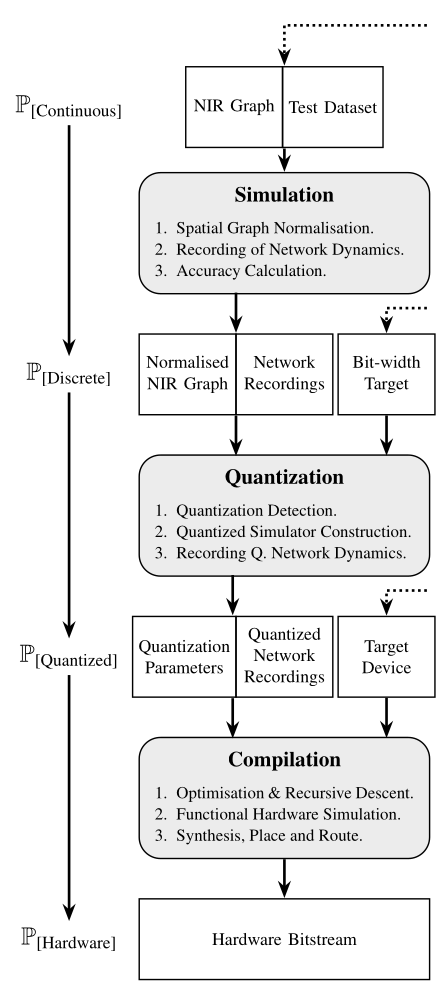
\includegraphics[width=3cm]{img/toolchain.png}
    \end{column}
  \end{columns}
\end{frame}

\begin{frame}{Theory}
  \begin{columns}
    \begin{column}{.5\textwidth}
      We make the definitions
      \begin{itemize}[<+->]
      \item A \textbf{primitive} $p \in \mathbb{P}$ is defined by its inputs, parameters, bounding differential equations and outputs.
      \item A \textbf{computational model} $\mathcal{M}$ specifies what regime primitive $p$ is evaluated in, for example: \emph{ODE}, \emph{Discrete} equation, \emph{Quantized} equation with discrete model, or in a digital \emph{Circuit}.
      \item A \textbf{primitive mapping} $\mathbb{P}_{[\mathcal{C}]}$ maps a primitive set $\mathbb{P}$ into a computational model $\mathcal{M}$.
      \end{itemize}
    \end{column}
    \begin{column}{.5\textwidth}
      \centering
    \end{column}
  \end{columns}
\end{frame}

\begin{frame}[fragile]{Theory}
  \begin{columns}
    \begin{column}{.5\textwidth}
      We make the definitions
      \begin{itemize}
      \item A \textbf{primitive} $p \in \mathbb{P}$ is defined by its inputs, parameters, bounding differential equations and outputs.
      \item A \textbf{computational model} $\mathcal{M}$ specifies what regime primitive $p$ is evaluated in, for example: \emph{ODE}, \emph{Discrete} equation, \emph{Quantized} equation with discrete model, or in a digital \emph{Circuit}.
      \item A \textbf{primitive mapping} $\mathbb{P}_{[\mathcal{C}]}$ maps a primitive set $\mathbb{P}$ into a computational model $\mathcal{M}$.
      \end{itemize}
    \end{column}
    \begin{column}{.5\textwidth}
      \centering
      The paper aims to implement the transformation
      \begin{equation*}
        {\mathbb{P}_{[ODE]}} \to {\mathbb{P}_{[Circuit]}}
      \end{equation*}

      \pause
        \vspace{0.5em}
        We model this as three separate unidirectional transformations
        \vspace{0.5em}

        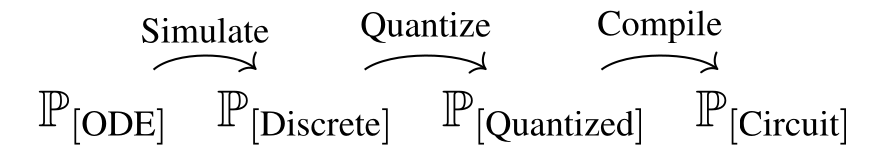
\includegraphics[width=\textwidth]{img/psmall.png}

    \end{column}
  \end{columns}
\end{frame}



\begin{frame}{Example Generation}
  \centering
  \foreach \n in {,1,2,3}{%
    \only<+>{\includegraphics[width=0.9\textwidth]{img/architecture\n.pdf}}%
  }
\end{frame}

% \begin{frame}{Preliminary Results}{}
%   {
%     \fontsize{8pt}{8pt}\selectfont
%     \begin{center}
\begin{tabular}{lllllrrr}
\hline
Network Representation & W/V Bits & Accuracy & Drop in Acc. & Time/Inf. & LUTs & DSPs & BRAMs\\
\hline
Sinabs Simulator & --- & 73.28\% & 0\% & --- & --- & --- & ---\\
\hline
NIR2FPGA (implicit support) & 16/16 & 63.56\% & -9.72\% & 7211us & 2386 & 24 & 38\\
NIR2FPGA (implicit support) & 8/8 & 55.67\% & -17.61\% & 6981us & 1935 & 16 & 20\\
\hline
\hline
SNNTorch & --- & 75.44\% & 0\% & --- & --- & --- & ---\\
Spiker+ & 5/6 & 72.99\% & -2.45\% & 540us & 18268 & 0 & 51\\
\hline
\end{tabular}
\end{center}

%%% Local Variables:
%%% mode: LaTeX
%%% TeX-master: t
%%% End:

%   }

%   \vspace{2em}
%   \begin{itemize}
%   \item Not great, but the upside is this heavily depends on FPGA implementation.
%   \item High discrepancy justifications (and things we plan on adressing):
%     \begin{itemize}
%     \item No formal verification of primitive hardware units.
%     \item Lack of thorough equivalence testing (we base on one sample).
%     \item Basically, we're not testing as much as we should.
%     \end{itemize}
%   \item MNIST LIF network results are slightly better: $-0.94\%$ for 16 bits, $-5.08\%$ for 8 bits.
%   \end{itemize}
% \end{frame}

\begin{frame}[allowframebreaks]{References}
    \AtNextBibliography{\tiny}
    \printbibliography
  \end{frame}

\end{document}
%%% Local Variables:
%%% mode: latex
%%% TeX-master: t
%%% End:
